% ############ 5.3) TEST PLAN ########################

In Microservice Architecture, testing is a critical aspect of software development since the fragmented structure increases the overall complexity of the system.
To have a better understanding of the problem, we can refer to Mike Cohn’s test pyramid (Fig. \ref{fig:test_pyramid}): as we move towards the top layers of the pyramid, the scope of the tests increases and the number of tests that must be written decreases.

\begin{figure}[H]
	\centering
    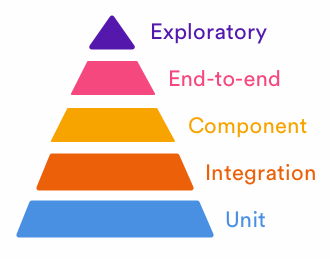
\includegraphics[scale=0.4]{Images/Impl, Integr & Test/test_pyramid.png}
	\caption{\label{fig:test_pyramid}Mike Cohn's test pyramid}
\end{figure}

Following this structure, we can identify different testing types:
\begin{itemize}
    \item unit testing
    \item integration testing
    \item component testing
    \item end-to-end testing
    \item performance testing
\end{itemize}

Unit testing is very important in this context to validate each business logic (aka microservice) separately, since it provides the coverage of each module in the system in isolation. It is better to keep the testing units as small as possible: it becomes easier to express the behavior if the test is small since the branching complexity of the unit is lower. Also, Unit testing is a powerful design tool when combined with Test-Driven Development (TDD).
\newline

Integration testing verifies the communication path and interactions between the components to detect interface defects. Integration test collects microservices together to verify that they collaborate as intended to achieve some larger piece of business logic.
One of the most important aspects of service-to-service testing is tracing, especially when multiple services are touched by a single test. Therefore, it becomes imperative to have observability and monitoring of requests across services.
\newline

Component testing is used to test single microservices in isolation, once we have executed unit tests of all the functions within microservices. Component tests should be implemented within each microservice’s code repository. By writing the test at the granularity of the microservices layer, the API behavior is driven through the test from the consumer perspective. At the same time, the component tests will test the interaction of microservices with the database, all as one unit.
\newline

End-to-end testing treats the system as a black box since its intention is to verify that the system as a whole meets business goals, irrespective of the component architecture in use. It provides coverage of the gaps between the services and, additionally, allows testing the  correctness of message passing between them. End-to-end testing is crucial to verify that the system is able to achieve the high-level functionalities it has been designed for.
\newline

Performance testing is the most complex testing strategy because of the high number of moving parts and supporting services/resources. However, performance load tests are crucial to understand how well the system can manage a wide set of users, especially in order to guarantee high availability and scalability.
\newline

In addition, it is highly suggested the adoption of Contract Testing every time an element relies on another element’s interface, in this case microservices. Having well-formed contract tests makes it easy for developers to avoid many problems in such a complex type of architecture, assuring easy development and deployment.
\newline

Moreover, for client-side applications (web app, mobile app), it is important to mention that some sort of acceptance testing should be taken into account, for example using the user experience feedback to do a validation of the design activity. This aspect is particularly important if a future transition to micro front-ends is going to take place: in fact, the user experience feedback will be a crucial element to consider when testing the client-side functionalities.
\newline

Finally, since the S2B will follow the Digital Public Good principles, special attention must be given to security aspects. In fact, they should be carefully tested in order to satisfy the constraints defined by India’s Personal Data Protection Act (PDPA), a set of regulations derived from the European General Data Protection Regulation (GDPR).
